% Auto-generated by the analysis pipeline — do not edit
% y > 0: Overreacts  |  y < 0: Underreacts
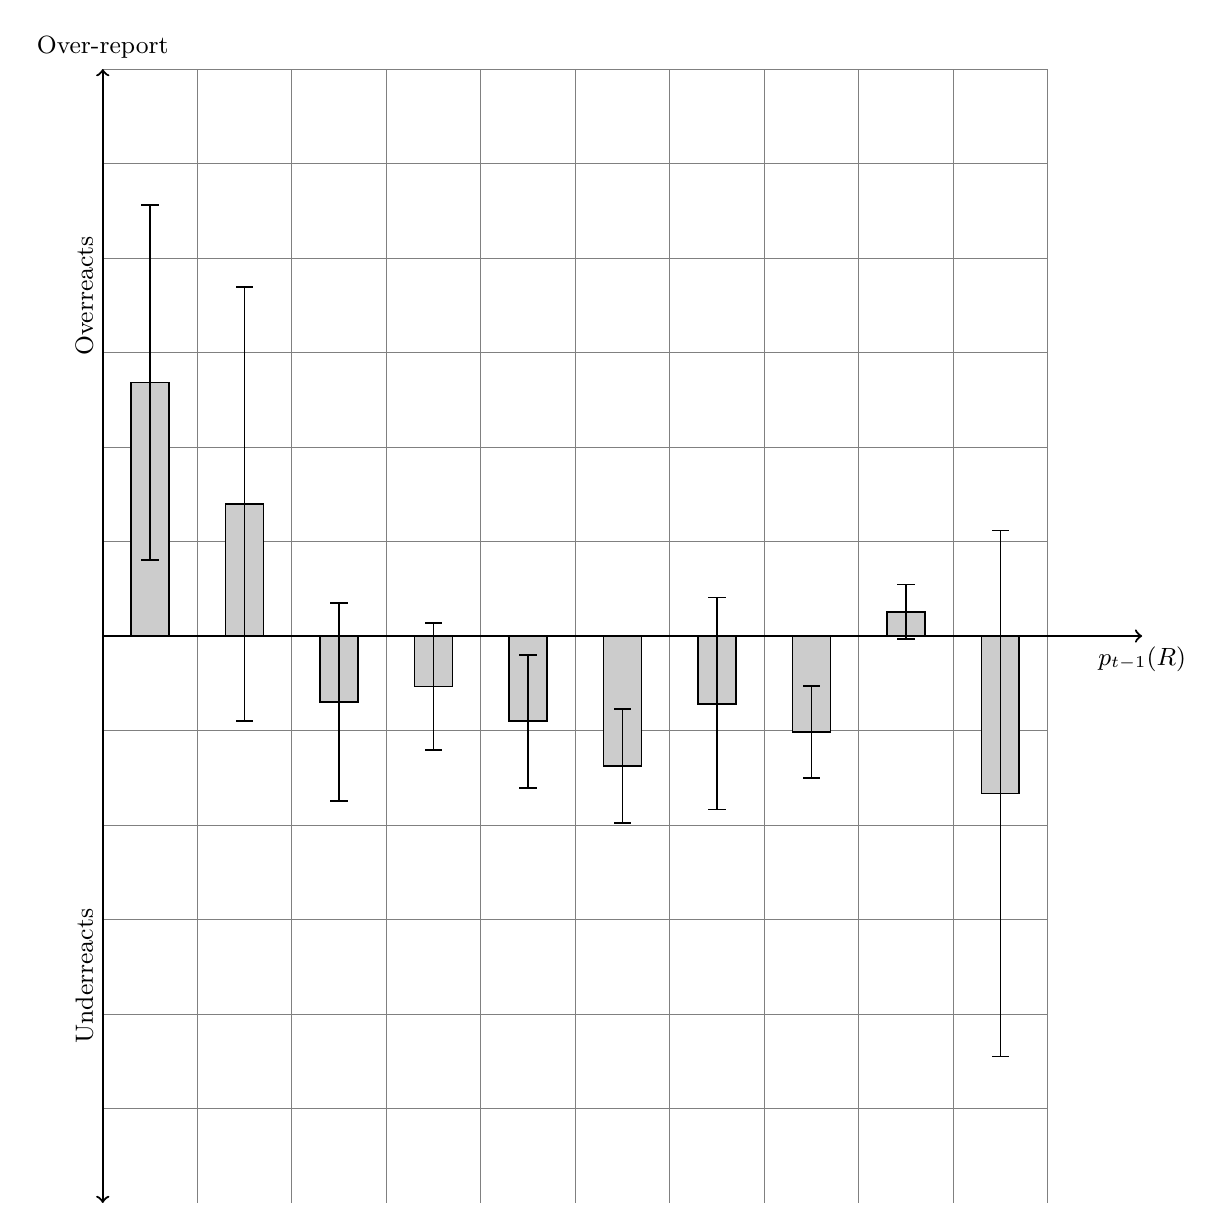
\begin{tikzpicture}[scale=12]
\draw[help lines,step=0.1] (0,-0.6) grid (1,0.6);
\filldraw[opaque,white!80!black] (0.03,0) rectangle (0.07,0.2683);
\draw[line width=0.6] (0.03,0) rectangle (0.07,0.2683);
\draw[line width=0.6,|-|] (0.05,0.0796) -- (0.05,0.4570);
\filldraw[opaque,white!80!black] (0.13,0) rectangle (0.17,0.1398);
\draw[line width=0.6] (0.13,0) rectangle (0.17,0.1398);
\draw[line width=0.6,|-|] (0.15,-0.0911) -- (0.15,0.3706);
\filldraw[opaque,white!80!black] (0.23,0) rectangle (0.27,-0.0697);
\draw[line width=0.6] (0.23,0) rectangle (0.27,-0.0697);
\draw[line width=0.6,|-|] (0.25,-0.1755) -- (0.25,0.0361);
\filldraw[opaque,white!80!black] (0.33,0) rectangle (0.37,-0.0534);
\draw[line width=0.6] (0.33,0) rectangle (0.37,-0.0534);
\draw[line width=0.6,|-|] (0.35,-0.1218) -- (0.35,0.0150);
\filldraw[opaque,white!80!black] (0.43,0) rectangle (0.47,-0.0901);
\draw[line width=0.6] (0.43,0) rectangle (0.47,-0.0901);
\draw[line width=0.6,|-|] (0.45,-0.1614) -- (0.45,-0.0189);
\filldraw[opaque,white!80!black] (0.53,0) rectangle (0.57,-0.1375);
\draw[line width=0.6] (0.53,0) rectangle (0.57,-0.1375);
\draw[line width=0.6,|-|] (0.55,-0.1989) -- (0.55,-0.0761);
\filldraw[opaque,white!80!black] (0.63,0) rectangle (0.67,-0.0716);
\draw[line width=0.6] (0.63,0) rectangle (0.67,-0.0716);
\draw[line width=0.6,|-|] (0.65,-0.1846) -- (0.65,0.0415);
\filldraw[opaque,white!80!black] (0.73,0) rectangle (0.77,-0.1015);
\draw[line width=0.6] (0.73,0) rectangle (0.77,-0.1015);
\draw[line width=0.6,|-|] (0.75,-0.1508) -- (0.75,-0.0523);
\filldraw[opaque,white!80!black] (0.83,0) rectangle (0.87,0.0256);
\draw[line width=0.6] (0.83,0) rectangle (0.87,0.0256);
\draw[line width=0.6,|-|] (0.85,-0.0043) -- (0.85,0.0555);
\filldraw[opaque,white!80!black] (0.93,0) rectangle (0.97,-0.1667);
\draw[line width=0.6] (0.93,0) rectangle (0.97,-0.1667);
\draw[line width=0.6,|-|] (0.95,-0.4458) -- (0.95,0.1124);
\draw[line width=0.8,->]  (0,0) -- (1.1,0) node[below] {\small{$p_{t-1}(R)$}};
\draw[line width=0.8,<->] (0,-0.6) -- (0,0.6) node[above] {\small{Over-report}};
\draw (0,0.36) node[above,rotate=90] {\small{Overreacts}};
\draw (0,-0.36) node[above,rotate=90] {\small{Underreacts}};
% ADD THEORY CURVE BELOW
\end{tikzpicture}
